% THIS IS SIGPROC-SP.TEX - VERSION 3.1
% WORKS WITH V3.2SP OF ACM_PROC_ARTICLE-SP.CLS
% APRIL 2009
%
% It is an example file showing how to use the 'acm_proc_article-sp.cls' V3.2SP
% LaTeX2e document class file for Conference Proceedings submissions.
% ----------------------------------------------------------------------------------------------------------------
% This .tex file (and associated .cls V3.2SP) *DOES NOT* produce:
%       1) The Permission Statement
%       2) The Conference (location) Info information
%       3) The Copyright Line with ACM data
%       4) Page numbering
% ---------------------------------------------------------------------------------------------------------------
% It is an example which *does* use the .bib file (from which the .bbl file
% is produced).
% REMEMBER HOWEVER: After having produced the .bbl file,
% and prior to final submission,
% you need to 'insert'  your .bbl file into your source .tex file so as to provide
% ONE 'self-contained' source file.
%
% Questions regarding SIGS should be sent to
% Adrienne Griscti ---> griscti@acm.org
%
% Questions/suggestions regarding the guidelines, .tex and .cls files, etc. to
% Gerald Murray ---> murray@hq.acm.org
%
% For tracking purposes - this is V3.1SP - APRIL 2009

\documentclass{acm_proc_article-sp}
\usepackage{float}

\begin{document}

\raggedbottom

\title{MPI NAS Parallel Benchmarks}
\subtitle{CSC 569}

\numberofauthors{4} 
\author{
\alignauthor
Ian Dunn\\
       \affaddr{Computer Science Department}\\
       \affaddr{Cal Poly}\\
       \affaddr{San Luis Obispo, California}\\
       \email{idunn01@calpoly.edu}
\alignauthor
Toshi Kuboi\\
       \affaddr{Computer Science Department}\\
       \affaddr{Cal Poly}\\
       \affaddr{San Luis Obispo, California}\\
       \email{tkuboi@calpoly.edu}
       \and % go to new row
\alignauthor
Mitchell Rosen\\
       \affaddr{Computer Science Department}\\
       \affaddr{Cal Poly}\\
       \affaddr{San Luis Obispo, California}\\
       \email{mwrosen@calpoly.edu}
\alignauthor
Austin Wylie\\
       \affaddr{Computer Science Department}\\
       \affaddr{Cal Poly}\\
       \affaddr{San Luis Obispo, California}\\
       \email{awylie@calpoly.edu}
}

\date{13 October 2013}

\maketitle
\begin{abstract}
Small abstract here.
\end{abstract}

\section{Setup}
Describe benchmarking process here.

\section{Results}
\subsection{Lab Machines}
Lab machine results here.

\subsection{Raspberry Pis}
Raspberry Pi results here.

Table~\ref{xmarkTable} shows \_.

\begin{table}[tbp]
\centering
\caption{XMark Test Results}
\label{xmarkTable}
\begin{tabular}{ c || c | c | c }

	Test & Tree & SAX & Diff\\ \hline
	01 & 0.003 & 0.003 & 0.000 \\
	02 & 0.091 & 0.054 & 0.037 \\
	03 & 0.180 & 0.104 & 0.076 \\
	04 & 0.354 & 0.206 & 0.148 \\
	05 & 0.434 & 0.261 & 0.173 \\
	06 & 0.520 & 0.296 & 0.224 \\
	07 & 0.682 & 0.392 & 0.290 \\
	08 & 0.861 & 0.509 & 0.352 \\
\end{tabular}
\end{table}

The graphs in Figures~\ref{tests001to008} through~\ref{tests201to210} also show \_.

\begin{figure}[tbp]
  \centering
  \caption{XMark Test Results (1 to 8)}
	\label{tests001to008}
  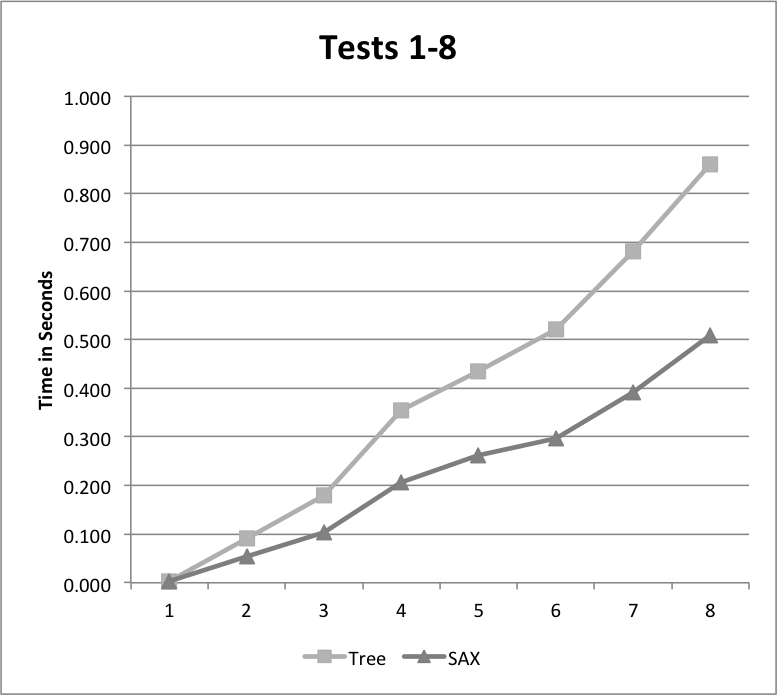
\includegraphics[width=20pc]{Tests001to008.png}
\end{figure}

\begin{figure}[tbp]
  \centering
  \caption{XMark Test Results (101 to 115)}
	\label{tests101to115}
  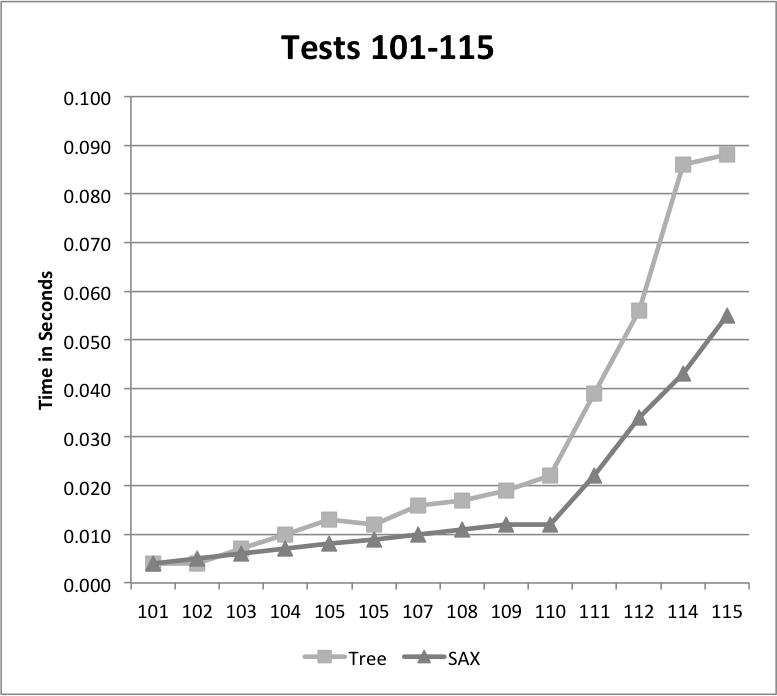
\includegraphics[width=20pc]{Tests101to115.png}
\end{figure}

\begin{figure}[tbp]
  \centering
  \caption{XMark Test Results (201 to 210)}
	\label{tests201to210}
  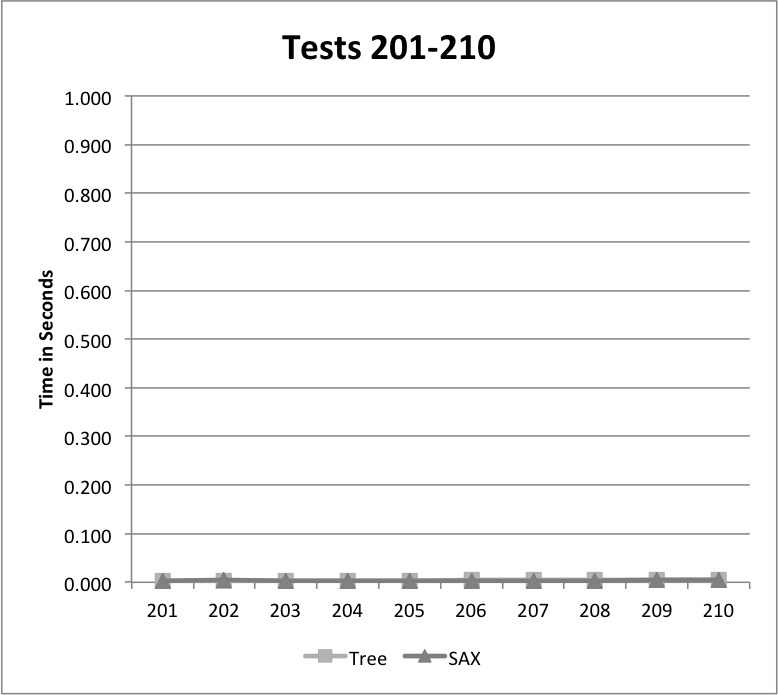
\includegraphics[width=20pc]{Tests201to210.png}
\end{figure}

Table~\ref{stressTable} outlines \_.

\begin{table}[tbp]
\centering
\caption{Stress Test Results}
\label{stressTable}
\begin{tabular}{ c || c | c }

	Test & Tree & SAX\\ \hline
	SWISS-PROT & 2.921 & 1.628\\
	PIR & Not Available & 12.758\\

\end{tabular}
\end{table}

\section{Analysis}
Analysis here.

\bibliographystyle{abbrv}
%\bibliography{sample}

%\balancecolumns 

\end{document}
